\documentclass{beamer}
\usepackage[utf8]{inputenc}

\usetheme{Madrid}
\usecolortheme{default}
\usepackage{tikz}
\usepackage{graphicx}
\usepackage{transparent}
\usetikzlibrary{calc}
\usepackage{subfiles}

%------------------------------------------------------------
%This block of code defines the information to appear in the
%Title page
\title[] %optional
{An introduction to hidden Markov models and their use for understanding animal movement}
\date{}

\author[Lambert] % (optional)
{Ben Lambert}



%End of title page configuration block
%------------------------------------------------------------



%------------------------------------------------------------
%The next block of commands puts the table of contents at the 
%beginning of each section and highlights the current section:-----------------------------------------------------------


\AtBeginSection[]
{
  \begin{frame}
    \frametitle{Current topic}
    \tableofcontents[currentsection]
  \end{frame}
}

\usepackage{xparse}

\let\oldquote\quote
\let\endoldquote\endquote

\RenewDocumentEnvironment{quote}{om}
  {\oldquote}
  {\par\nobreak\smallskip
   \hfill#2\IfValueT{#1}{, #1}\endoldquote 
   \addvspace{\bigskipamount}}

\usepackage{amsmath}
\DeclareMathOperator*{\argmax}{arg\,max}

\begin{document}

%The next statement creates the title page.
\frame{\titlepage}

\subfile{introduction_inference_problem}

\subfile{forward}

\subfile{viterbi}

\begin{frame}
\frametitle{Elephants revisited}

\begin{figure}
    \centering
    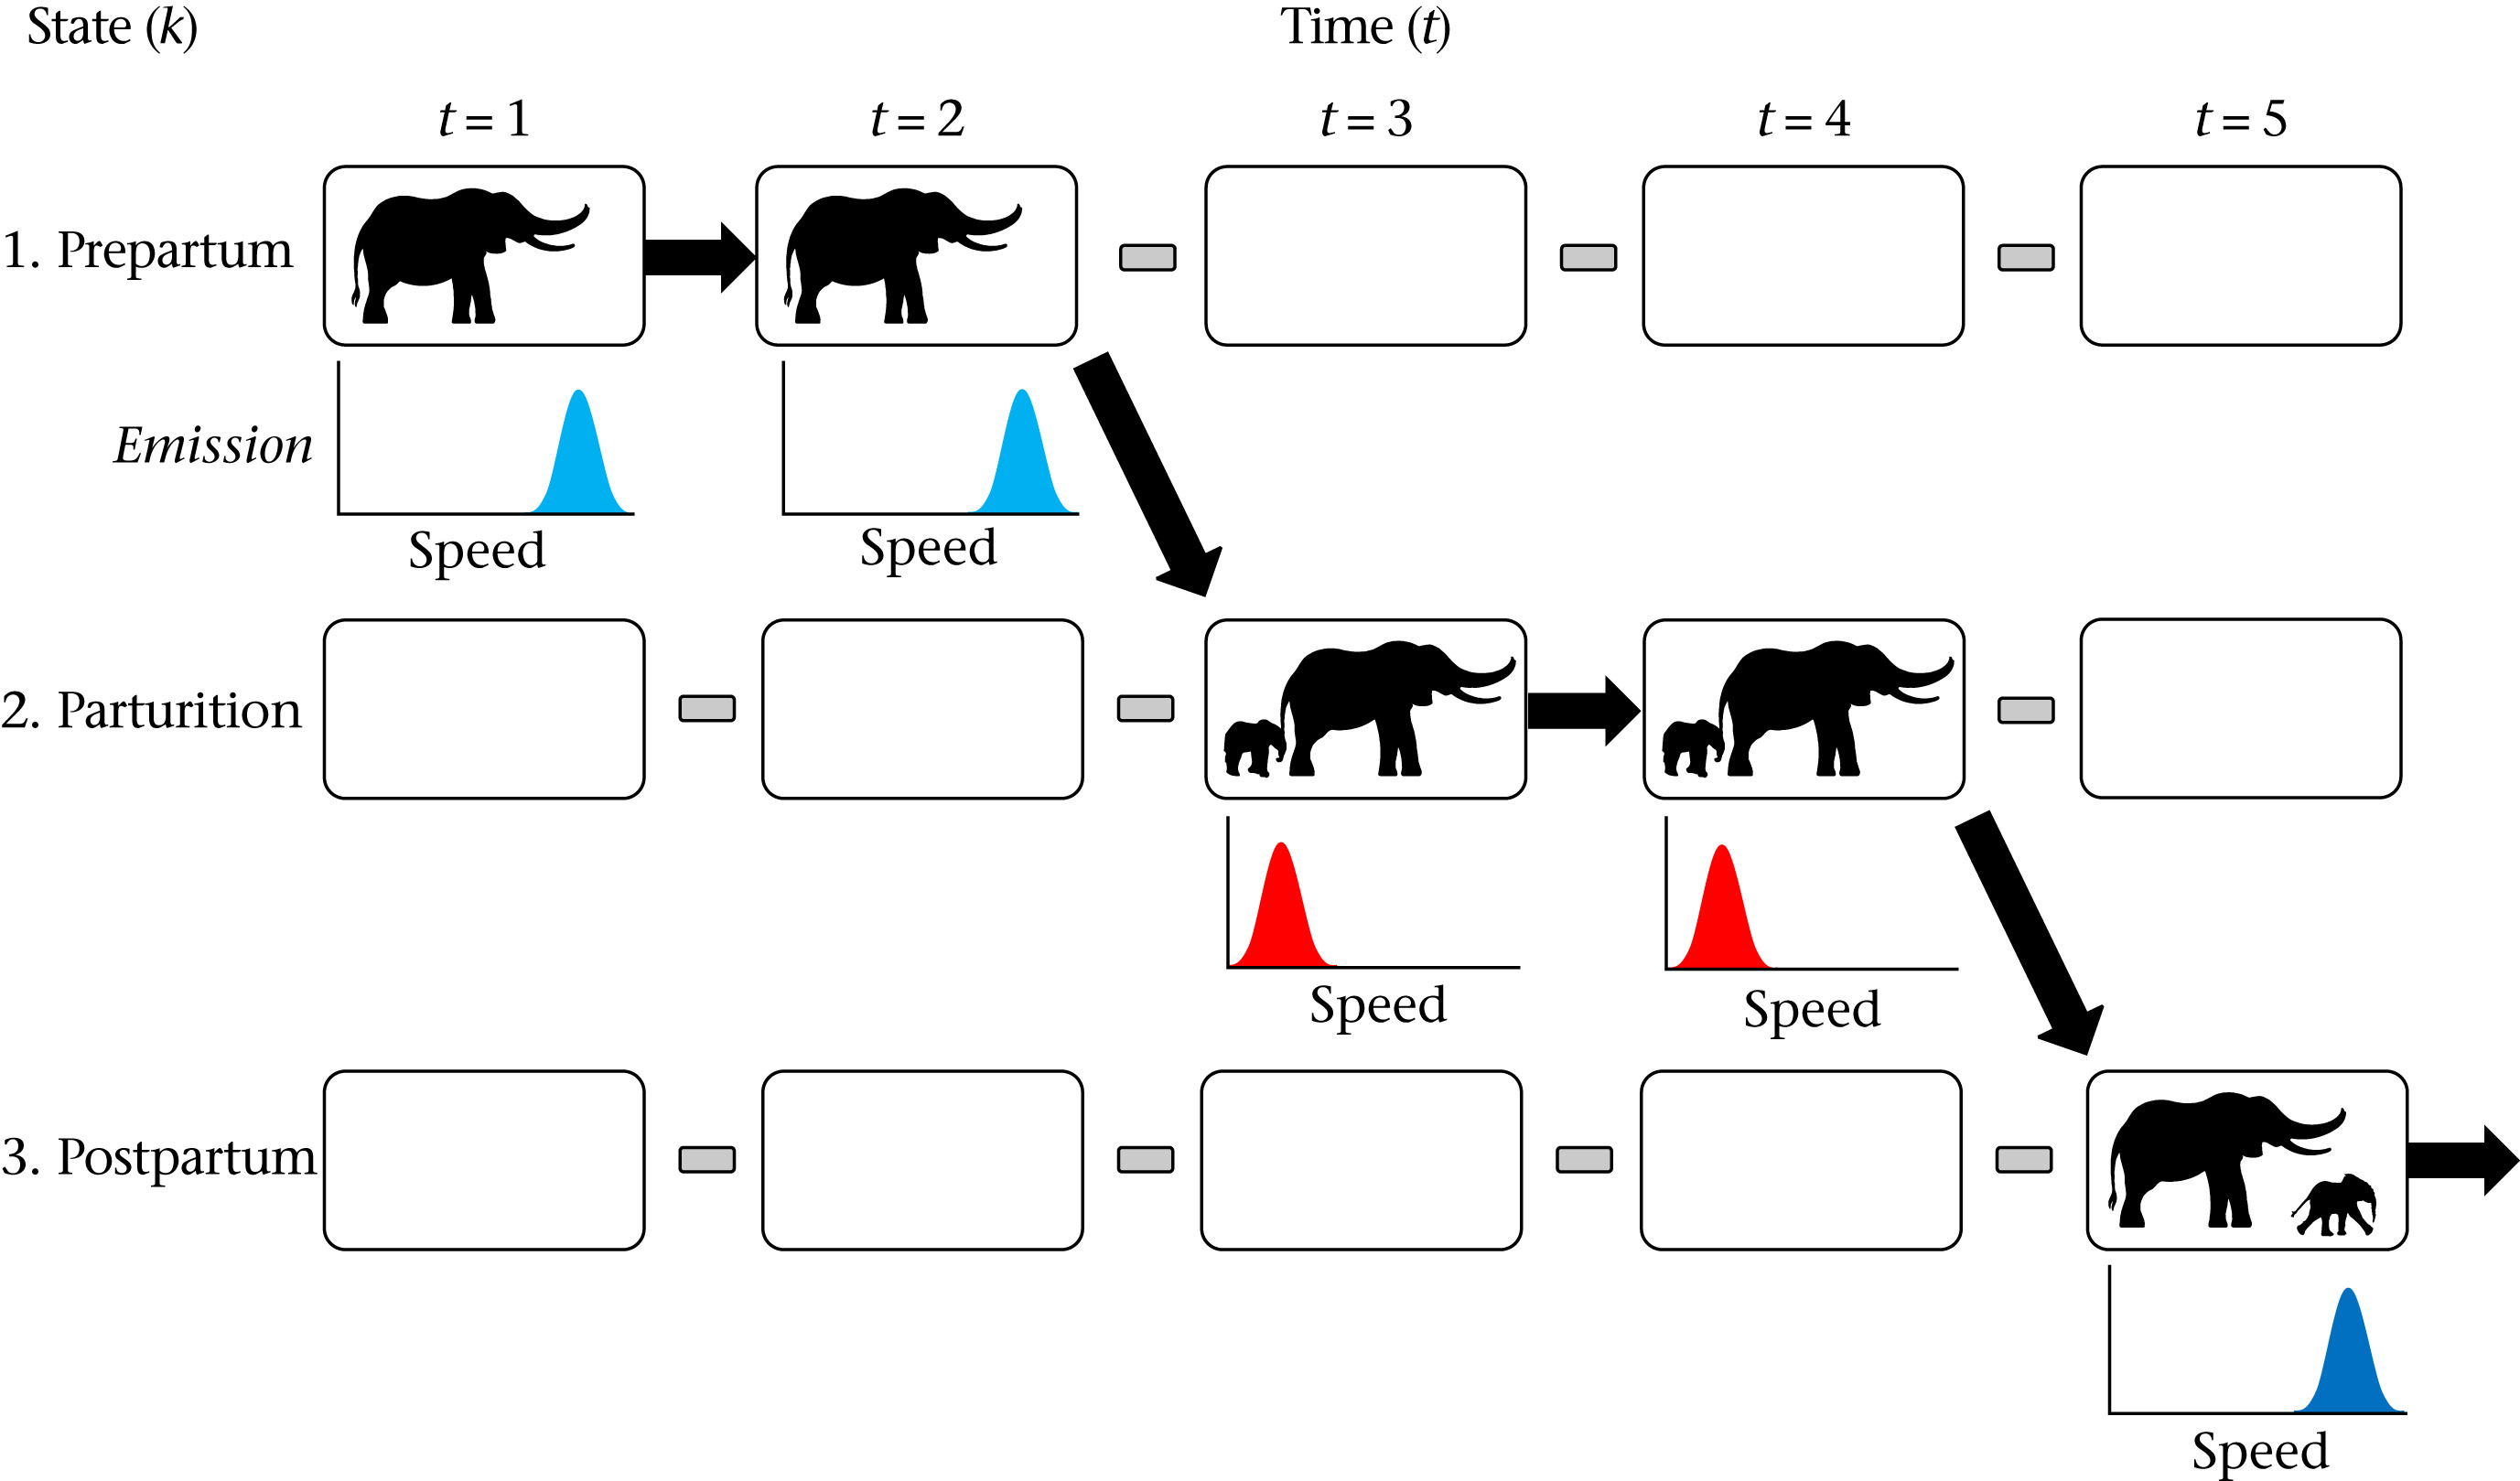
\includegraphics[width=0.8\textwidth]{figures/elephant_parturition.jpg}
\end{figure}
    
\end{frame}

\begin{frame}
\frametitle{Study details}

\begin{itemize}
    \item 23 multiparous elephants
    \item 3 primiparous elephants
\end{itemize}

Used 2 month blocks of daily or hourly speed around estimated parturition date (how was this estimated?).

\vspace{0.5cm}

Model was fitted in a Bayesian framework using Stan.
    
\end{frame}

\begin{frame}
\frametitle{Multiparous females: 1}

\begin{figure}
    \centering
    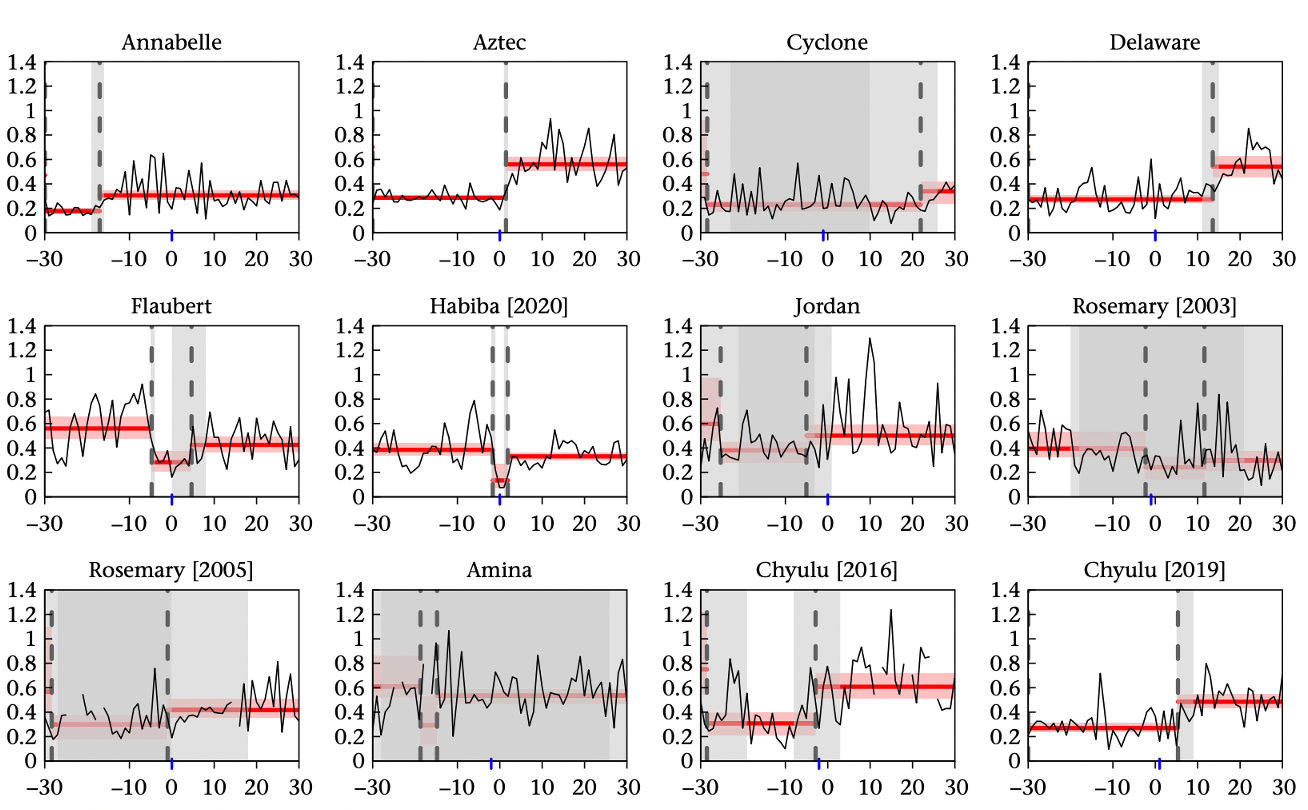
\includegraphics[width=0.9\textwidth]{figures/multiparous_1.png}
\end{figure}
    
\end{frame}

\begin{frame}
\frametitle{Multiparous females: 2}

\begin{figure}
    \centering
    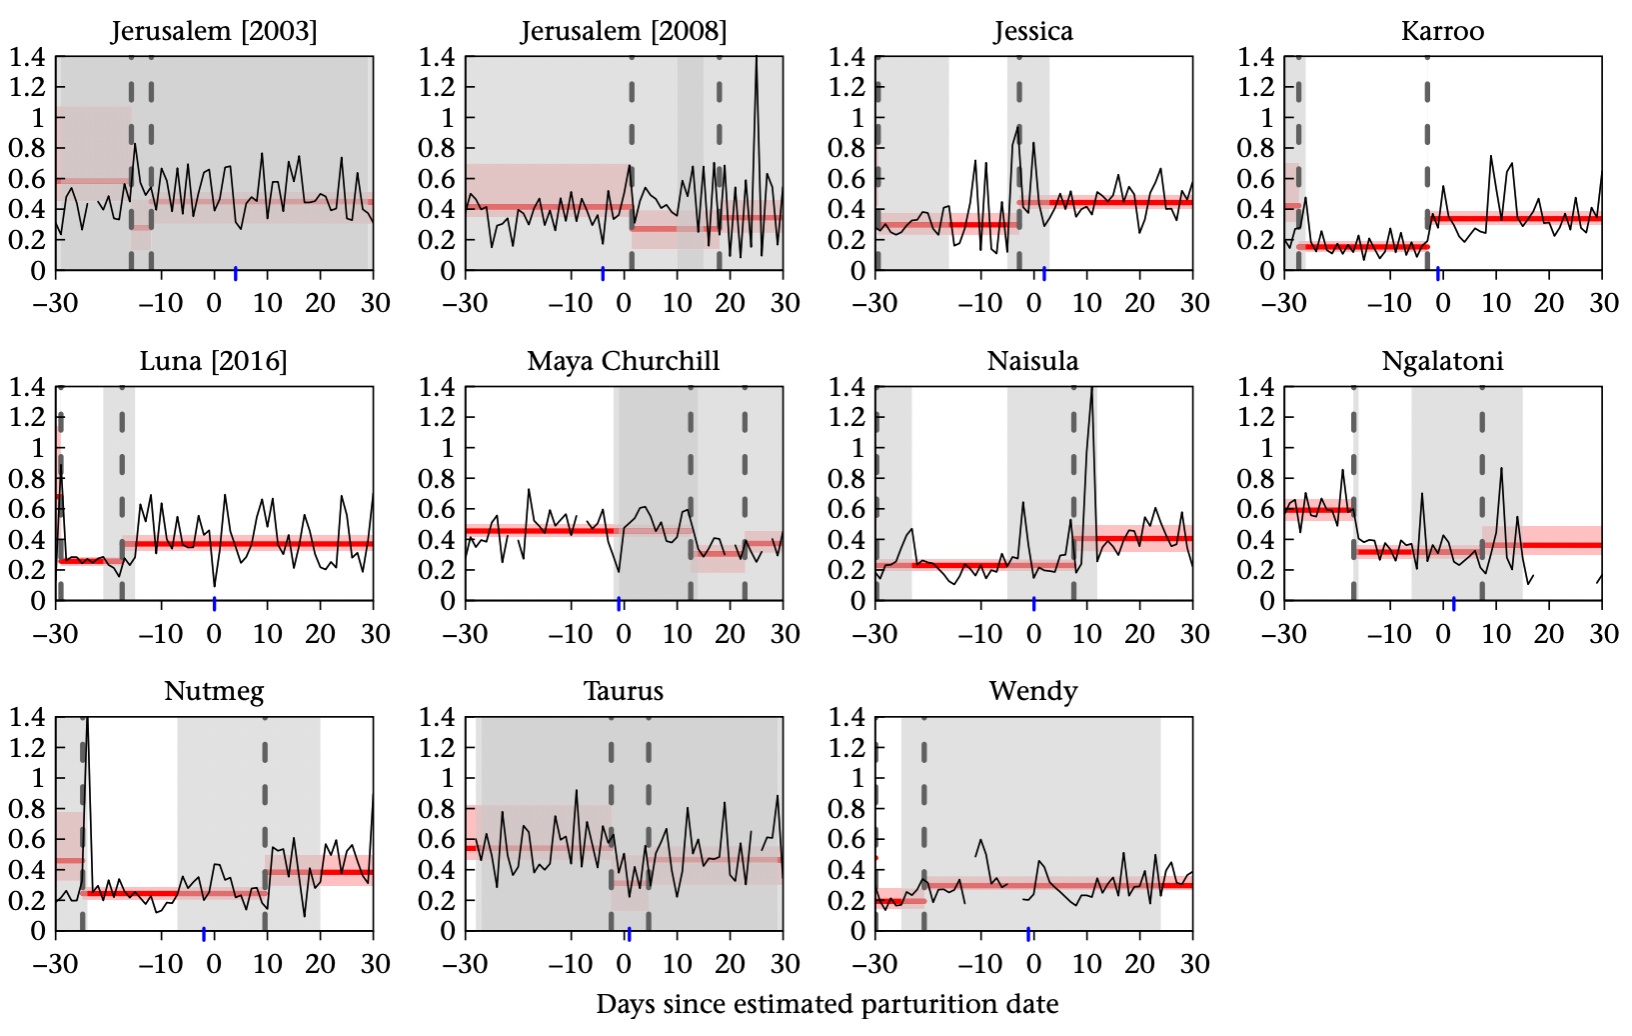
\includegraphics[width=0.9\textwidth]{figures/multiparous_2.png}
\end{figure}
    
\end{frame}

\begin{frame}
\frametitle{Primiparous females: e) Luna and f) Soutine}

\begin{figure}
    \centering
    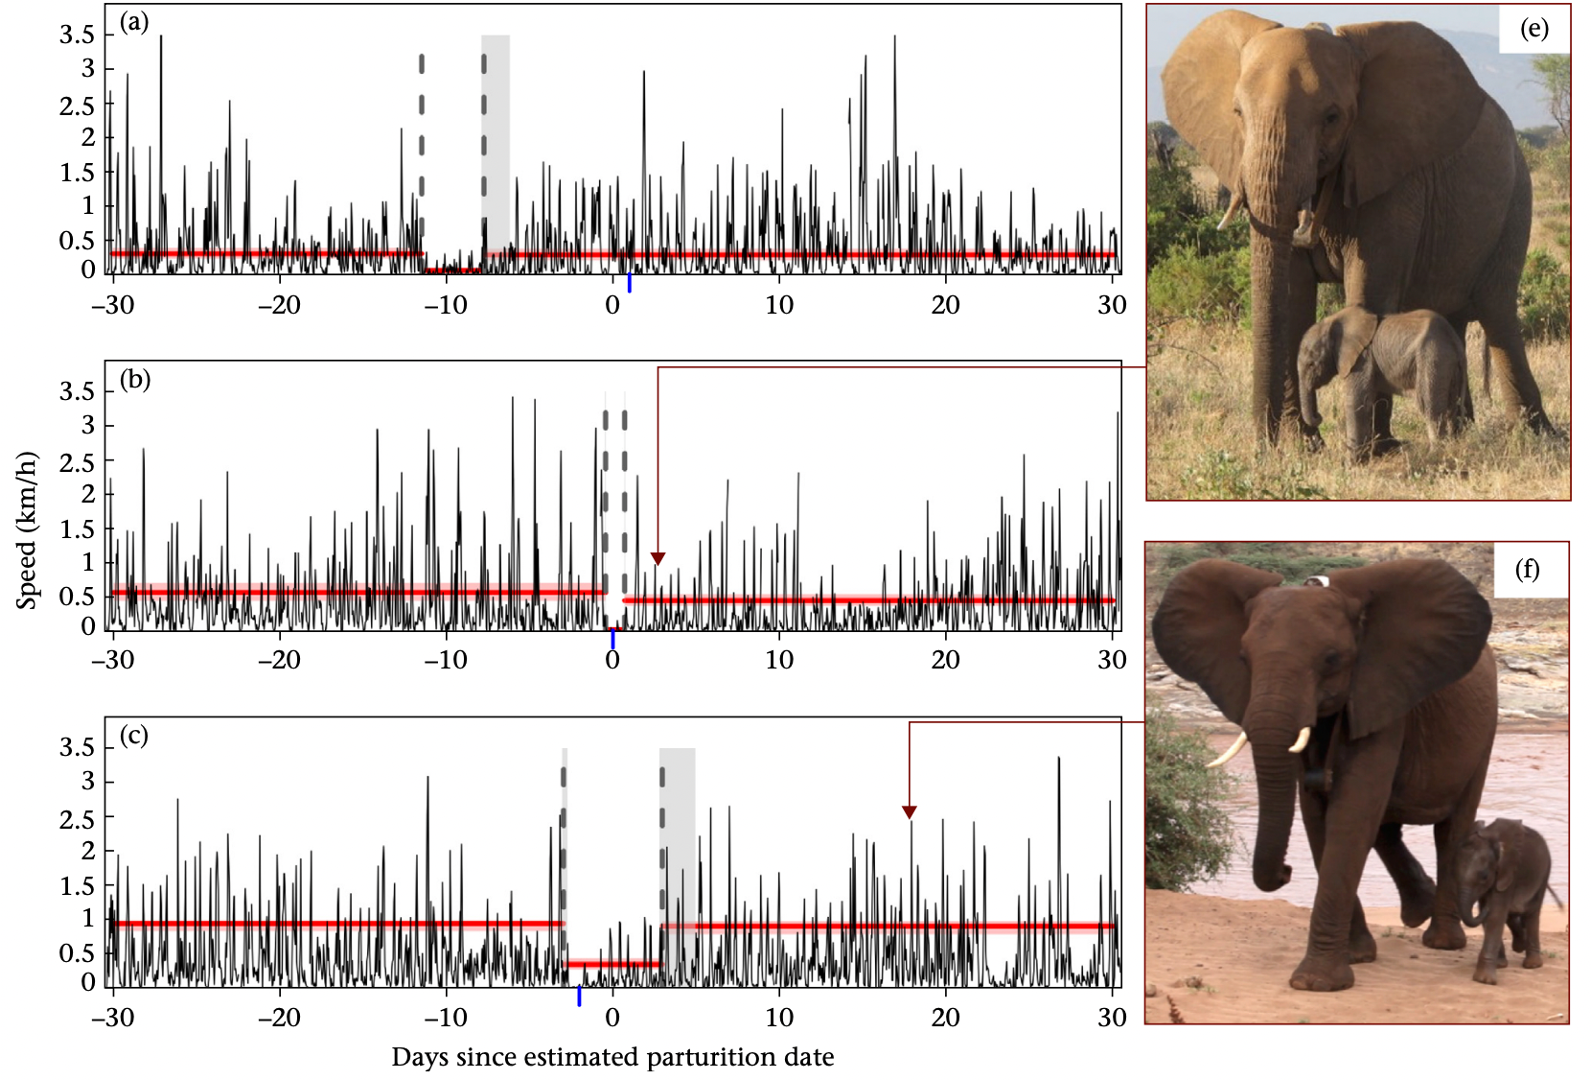
\includegraphics[width=0.85\textwidth]{figures/primiparous.png}
\end{figure}
    
\end{frame}

\begin{frame}
\frametitle{Parturition study conclusions}

\begin{itemize}
    \item Mixed effects linear models indicated that multiparous elephants decreased their speeds on estimated parturition date
    \item But we only detected parturition in 4 / 23 multiparous females
    \item In our sample of 3 primiparous elephants, we detected the known parturition date in 2 / 3
\end{itemize}

\vspace{0.5cm}

Overall, remarkably undetectable changes in speed around birth.

\vspace{0.5cm}

The precocial abilities of calves facilitate the maintenance of group cohesion and elephants may have evolved a long
gestation period to facilitate an advanced stage of fetal physical development.
    
\end{frame}

\begin{frame}
\frametitle{Conclusions}

\begin{itemize}
    \item HMMs assume persistent latent behaviours drive differences in observations
    \item Efficient algorithms exist for fitting these models to data
    \item HMMs do not replace fieldwork and ecological know-how
    \item Indeed field insights are often essential to effective use of these powerful tools
\end{itemize}
    
\end{frame}

\end{document}